% !TEX root = /Users/hzd88688126com/Desktop/USFD_Academic-_Report_LaTeX-Template/main.tex
\section{Periodogram-based Methods Applied to Real-World Data}
\subsection{The sunspot time series}
As shown in Fig.\ref{fig:1_2_a}, the periodograms of raw sunspots data and its processed data are compared, including \texttt{detrend} in red line, \texttt {mean} in orange and \texttt {logarithm} in purple. In addition, the effects of applying rectangular window and Hanning window on spectral are illustrated as well. 
\begin{figure}[htbp]
     \centering
      \hspace{-0.4cm}
     \begin{subfigure}[b]{0.33\textwidth}
         \centering
         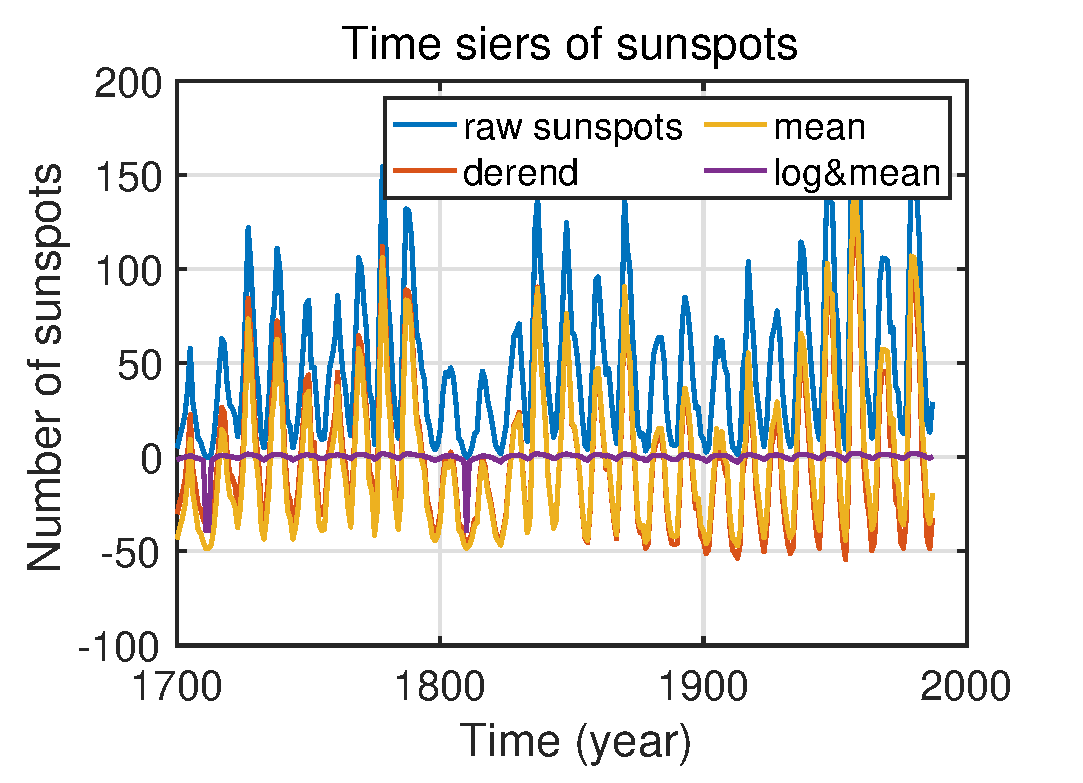
\includegraphics[width=\textwidth]{fig/12/12a1.eps}
         \caption{Time series}
         \label{fig:raw}
     \end{subfigure}
      \hspace{-0.4cm}
     \begin{subfigure}[b]{0.33\textwidth}
         \centering
         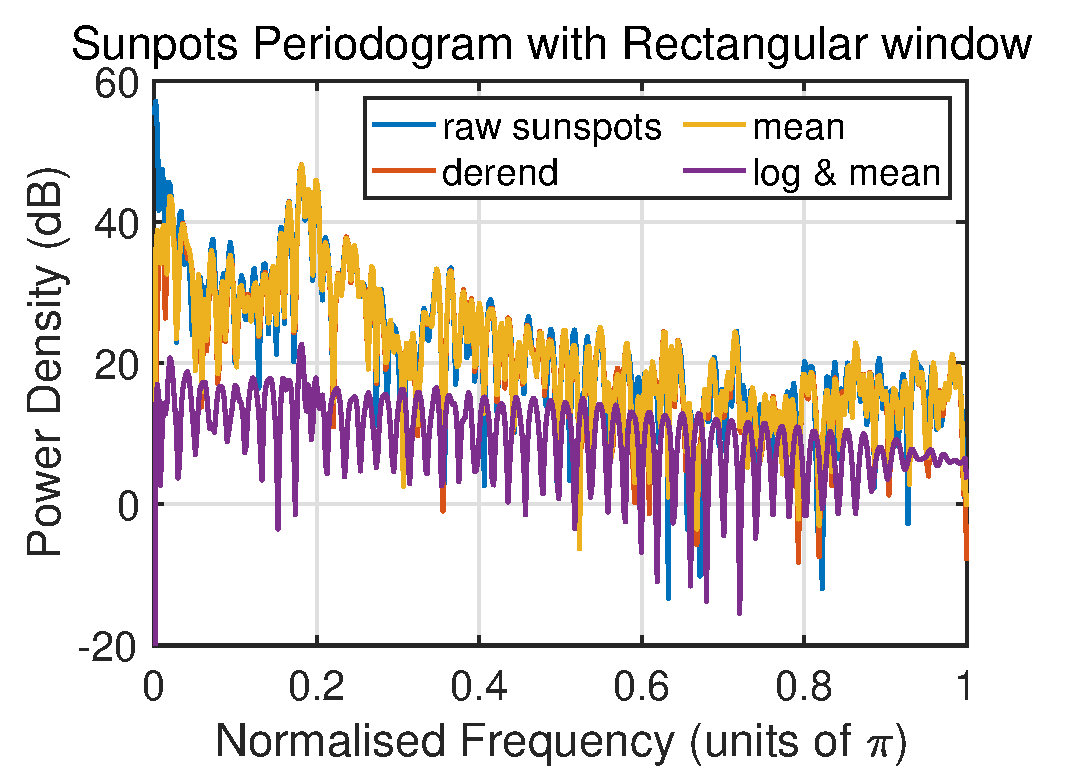
\includegraphics[width=\textwidth]{fig/12/12a2.eps}
         \caption{Rectangular window}
         \label{fig:rect}
     \end{subfigure}
      \hspace{-0.4cm}
     \begin{subfigure}[b]{0.33\textwidth}
         \centering
         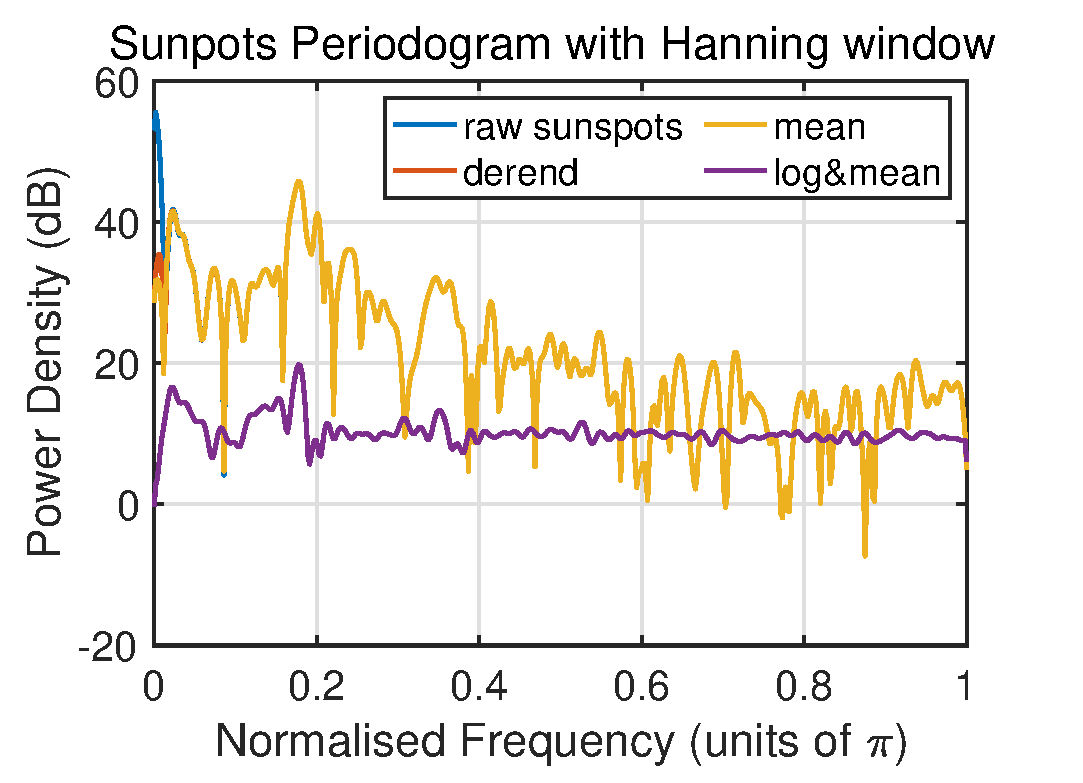
\includegraphics[width=\textwidth]{fig/12/12a3.eps}
         \caption{Hanning window}
         \label{fig:hann}
     \end{subfigure}
        \caption{Periodogram of processing sunspots data with rectangular and Hanning window}
        \label{fig:1_2_a}
\end{figure}\\
The results of using \texttt{detrend} and \texttt{mean} are similar. However, subtracting its mean leads to removing the DC component in zero frequency, while \texttt{detrend} results in eliminating the linear trend of a vector under low frequency region. Afterwards, the PSD curves of processing and raw data are same. As to centring after \texttt{log}, the curve is smoothly and the variance is reduced, as consequence of that the peaks are difficult to be detected.\\
Applying different windows will cause the changing of periodogram, due to the resolution of mainlobe width and sidelobe attenuation. Compared with Fig.\ref{fig:rect} and \ref{fig:hann}, the curve is smoothly with less ripples when using the Hanning window. The reason is that the Hanning window has larger mainlobe width than rectangular window. Moreover, interest peaks can be effectively detected by applying \texttt{log}, since most of ripples are eliminated.
\subsection{The basis for brain computer interface (BCI)}
Fig.\ref{fig:1_2_b1} illustrates periodagrams of the standard and Bartlett method. By applying Bartlett averaging method, the peaks of frequency are easily detected which are the range of $8-10$, $13$, $26$, $39$ and $50$ $Hz$. As stated in instruction, the strong response within $8-10 \ Hz$ and $50 \ Hz$ are not the SSVEP\cite{mandic}. Therefore, the fundamental frequency peak of the SSVEP is at $f=13 \ Hz$ with harmonics frequencies at $f=26 \ Hz$ and $f=39 \ Hz$.
\begin{figure}[htp]
     \centering
     \begin{subfigure}{0.4\textwidth}
         \centering
         \includegraphics[width=\textwidth]{fig/12/12b1.eps}
     \end{subfigure}
     ~
     \begin{subfigure}{0.4\textwidth}
         \centering
         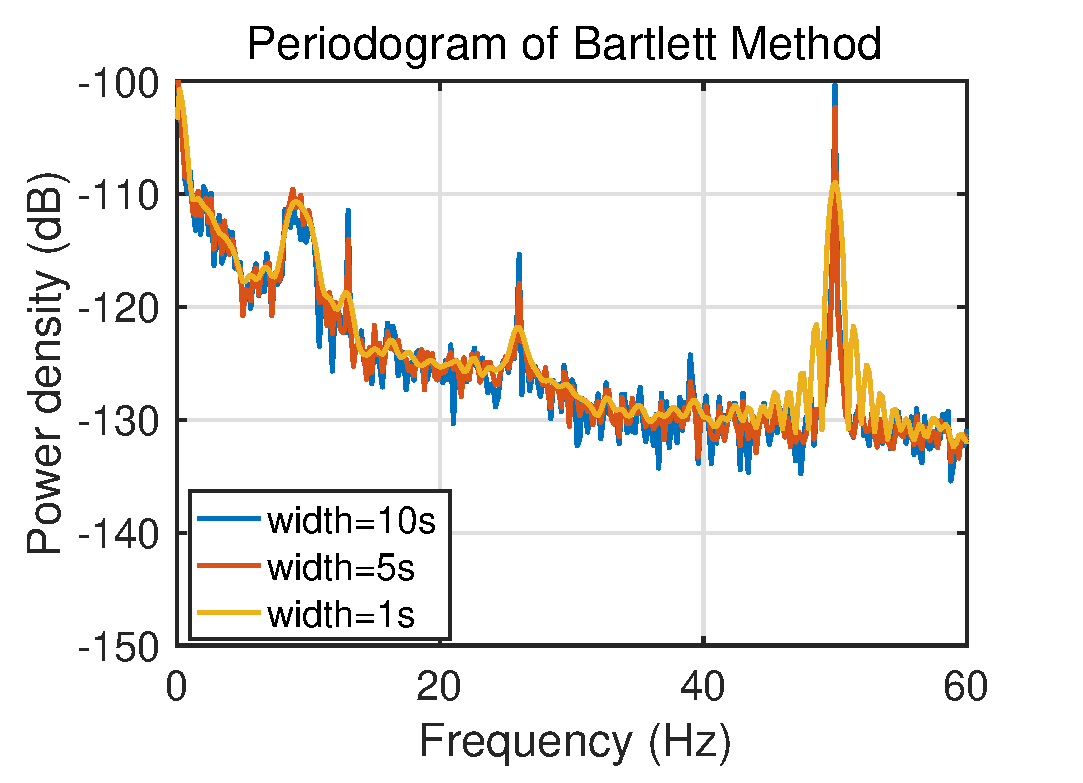
\includegraphics[width=\textwidth]{fig/12/12b2.eps}
     \end{subfigure}
        \caption{Standard and Bartlett Method of EEG Periodograms}
        \label{fig:1_2_b1}
\end{figure}\\
With different length of windows, the total signal is divided into different length of segments. Fig.\ref{fig:1_2_b2} depicts the different periodograms with lengths of $\Delta t=10s$ and $\Delta t=1s$ windows. As to $\Delta t=1s$, the periodogram is smooth with reduced variance. Nevertheless, the peak frequencies of interest are unapparent resulting in difficultly detecting the SSVEP\cite{mandic}. Only alpha-rhythm peak at 8-10 $Hz$ and interference at 50 $Hz$ can be observed. When increasing the window length such as $\Delta t =10s$, the number of segments decreases and each segment is longer. Hence, the variance of periodogram is reduced to a slight extent, resulting in distinct peak. However, the variance is sufficiently elimanitade compared with standard periodogram. Therefore, the trade-off between variance and precision need to be considered. 
\begin{figure}[htp]
     \centering
     \begin{subfigure}{0.4\textwidth}
         \centering
         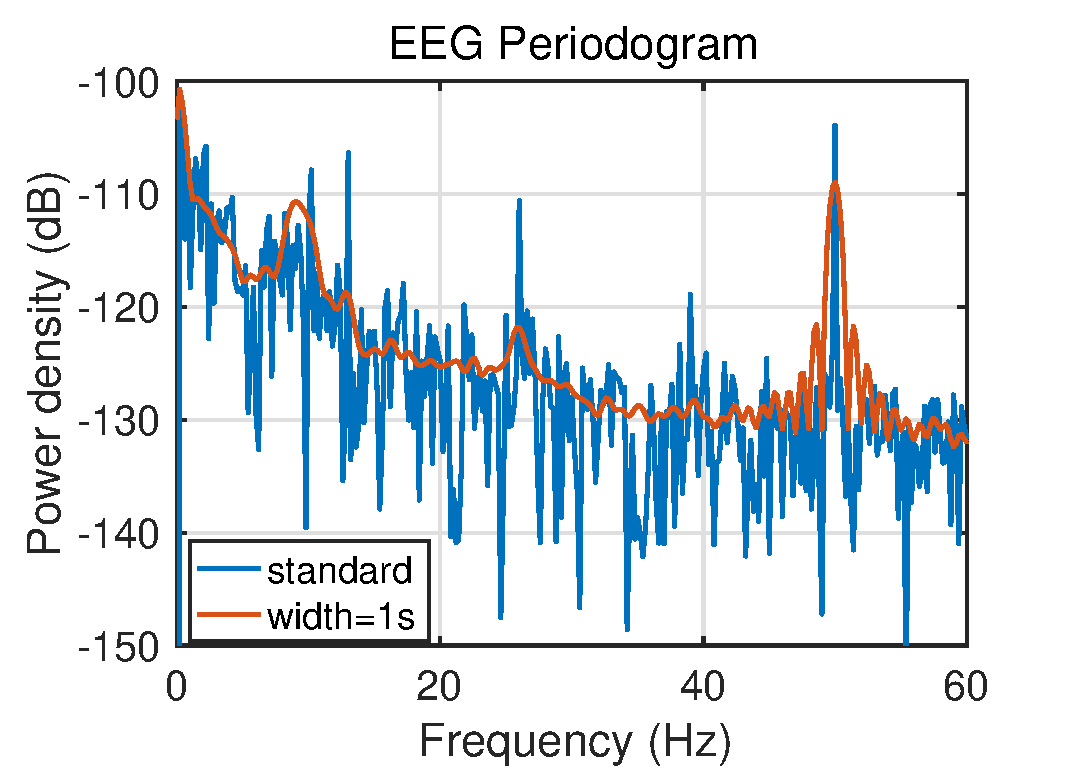
\includegraphics[width=\textwidth]{fig/12/12b4.eps}
     \end{subfigure}
     ~
     \begin{subfigure}{0.4\textwidth}
         \centering
         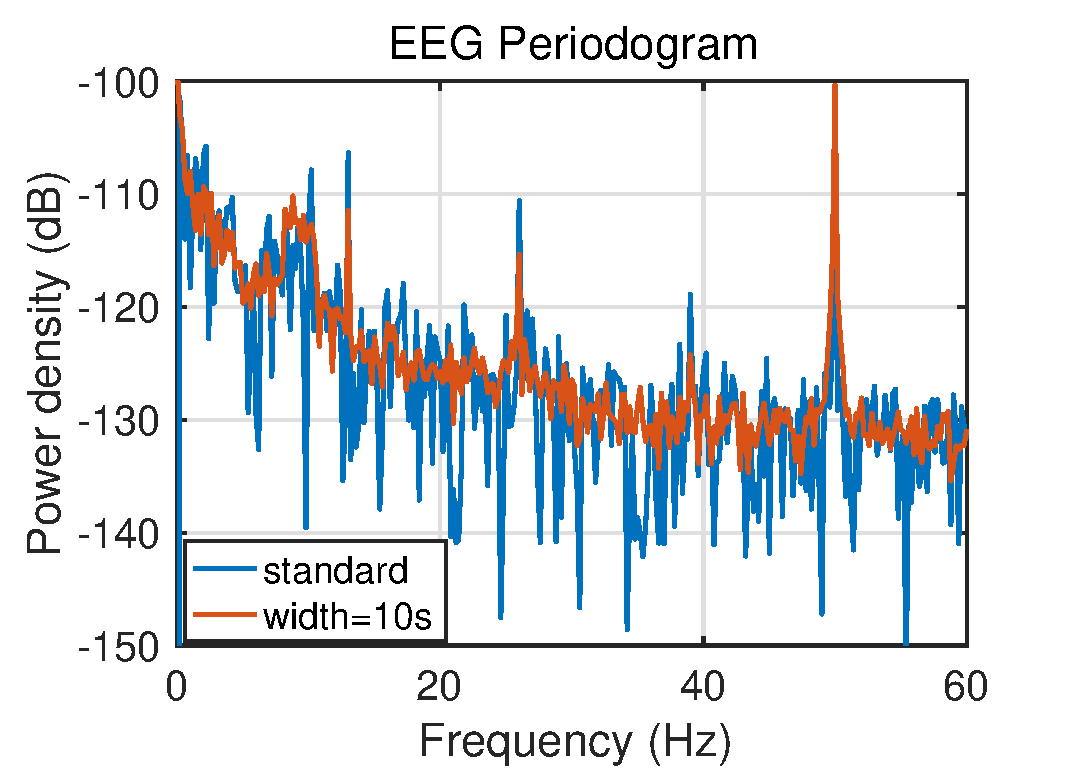
\includegraphics[width=\textwidth]{fig/12/12b3.eps}
     \end{subfigure}
        \caption{Bartlett method with different windows of EEG Periodograms}
        \label{fig:1_2_b2}
\end{figure}

